\subsection{Analyse af 2. orden lavpasfilter}

Figur \ref{2orden_ana} viser et 2. ordens lavpasfilter med en medstand, en spole og en kondensator.

$V_{in}$ er stepinput med spænding 0 - 5 V. Steppet sker til tiden t = 0 sek.

\begin{equation}
 V_{in}(t) =
  \begin{cases}
    0 & \quad \text{if } t <0\\
    V_{0}&\quad \text{if } t >0\\
  \end{cases}
  \label{V_in(t)2}\\
\end{equation}
\begin{center}

Ligning: \ref{V_in(t)2} Indgangs spændingen er en funktion af t
\end{center}

\begin{figure}[h]
 \begin{center}
  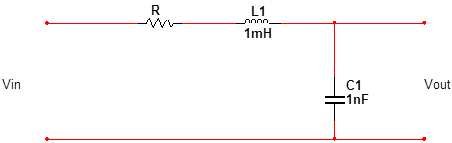
\includegraphics[height=2.5cm]{P_Fig/figur13_ana2}
  \caption{Anden ordens lavpasfilter}
  \label{2orden_ana}
 \end{center}
\end{figure}

\newpage

Strøm-spænding sammenhængen for en modstand, en spole og en kondensator er: \\

Modstand:
\begin{equation}
 V_{R} =R\cdot i
\label{Modstand2}\\
\end{equation}
\begin{center}
Ligning \ref{Modstand2}: Spændingen over en modstand
\end{center}

Spole:
\begin{equation}
	V_{L} = L\cdot \dfrac{d \c(i)}{dt}
\label{Spole2}\\
\end{equation}
\begin{center}
Ligning \ref{Spole2}: Spændingen over en Spole
\end{center}


Kondensator:
\begin{equation}
 i =C\cdot \frac{d(V_{C})}{dt}
\label{Kondensator2}\\
\end{equation}
\begin{center}
Ligning \ref{Kondensator2}: Strømmen gennem en kondensator
\end{center}

Output spænding:
\begin{equation}
V_{Out}(t) = V_{C}(t)
\label{V_out=V_C2}\\
\end{equation}
\begin{center}
Ligning \ref{V_out=V_C2}: Spændingen over $V_ {C}(t)$ er den samme som i punktet $V_{Out}(t)$
\end{center}

Følgende 7 delopgaver er givet:
\subsubsection*{1. Vis ved Kirchhoffs love : KVL}
Vis ved Kirchhoffs love at følgende differentialligning gælder for kredsløbet i Figur \ref{2orden_ana} : 

\begin{equation}
	L\cdot C\cdot \dfrac{d^{2}}{dt}\cdot V_{out}  \left(t\right) +R\cdot C\cdot \dfrac{d}{dt}\cdot V_{out}  \left(t\right) +V_{out}  \left(t\right)  = V_{in}  \left(t\right)
\label{dfLigning2}\\
\end{equation}

Efter en kredsløbsanalyse ses det at:
\begin{equation} V_{in}=V_{R}+V_L+V_{C}
\label{V_in:KVL2}
\end{equation}
 
 Ved brug af Ligning \ref{V_out=V_C2}  kan ligningen omskrives til 
\begin{equation}
V_{in}=V_{R} + V_L + V_{Out}
\label{V_0:KVL2}
\end{equation}

Ved at kombinere Ligning \ref{Modstand2} og Ligning \ref{Kondensator2}, samt Ligning \ref{Spole2} og Ligning \ref{Kondensator2} kan der findes et nyt udtryk fra $V_{R}$ og $V_L$ som er afhængig af tiden t
\begin{equation}
	V_{R} = R\cdot C\cdot \dfrac{d}{dt}\cdot V_C
\end{equation}

\begin{equation}
	V_{L} = L\cdot \dfrac{d}{dt} \cdot C\cdot \dfrac{d}{dt}\cdot V_C   
\end{equation}

Dernæst kan den indsættes i Ligning \ref{V_0:KVL2} hvilket medføre 
\begin{equation}
 V_{in}= R \cdot C \cdot \frac{d(V_{out}(t))}{dt} + L\cdot \dfrac{d}{dt} \cdot C\cdot \dfrac{d(V_{out}(t))}{dt} + V_{out}(t)
 \label{KVL2_2}
\end{equation}

Ligning \ref{KVL2_2} kan omskrives til:
\begin{equation}
	V_{in} = R\cdot C\cdot \dfrac{d}{dt}\cdot V_{out}+V_{out}+L\cdot C\ \dfrac{d^{2}}{dt^{2}}\ V_{out}
	\label{KVL2_3}
\end{equation}

\newpage

Ved at bytte rundt på rækkefølgen af Ligning \ref{KVL2_3}, kan den opstilles så den ligner Ligning \ref{dfLigning2}
\begin{equation}
	L\cdot C\cdot \dfrac{d^{2}}{dt^{2}}\cdot V_{out}  \left(t\right) +R\cdot C\cdot \dfrac{d}{dt}\cdot V_{out}  \left(t\right) +V_{out}  \left(t\right)  = V_{in}  \left(t\right)
	\label{KVL2_done} 
\end{equation}

\subsubsection*{2. Løs differentialligningen med hensyn til Vout }
 Løs differentialligningen med hensyn til $V_{out}$ for $ 0\leq t<\infty$ med hhv. R = 10k$\Omega$ og \\ R = 1k$\Omega$ \\

Vi har brugt brug af løsningsprotokolen for en 2. orden DL.

DL 2. orden for 10k$\omega$

1. Vores ligning \ref{KVL2_done} står allerede på den rigtige form, så ud fra denne ligning kan vi finde vores konstanter a, b, c og vores funktion f(t)

\begin{center}
\begin{minipage}{.2\linewidth}
a = L $\cdot$ C
\end{minipage}
\begin{minipage}{.2\linewidth}
b = R $\cdot$ C
\end{minipage}
\begin{minipage}{.2\linewidth}
c = 1
\end{minipage}
\begin{minipage}{.2\linewidth}
f(t) = $V_{in}(t)$
\end{minipage}
\end{center}

2. Find den homogene løsning: 
\begin{equation}
	L\cdot C\cdot \dfrac{d^{2}}{dt^{2}}\cdot V_{out}  \left(t\right) +R\cdot C\cdot \dfrac{d}{dt}\ V_{out}  \left(t\right) +V_{out} = 0
\end{equation}

2.1 opskriv karakterligningen:
\begin{equation}
	L\cdot C\cdot k^{2}+R\cdot C\cdot k+c = 0
\end{equation}

2.2 Løs karakterligningen

\begin{center}
\begin{minipage}{.2\linewidth}
R=10k$\Omega$
\end{minipage}
\begin{minipage}{.2\linewidth}
L = 1 mH
\end{minipage}
\begin{minipage}{.2\linewidth}
C = 1 nF
\end{minipage}
\end{center}

\begin{equation}
	k_{1} = \dfrac{ -R\cdot C+ \sqrt{ \left(R\cdot C\right) ^{2}-4\cdot L\cdot C\cdot 1} }{2\cdot L\cdot C} \rightarrow 
	\dfrac{2\cdot  \sqrt{25\cdot k^{\Omega}\cdot nF^{2}-nF\cdot mH} -10\cdot k\cdot nF}{2\cdot nF\cdot mH}
\end{equation}

$k_1$ = $\left( -1.01\cdot 10^{5}\right) \ \dfrac{1}{s}$

\begin{equation}
	k_{2} = \dfrac{ -R\cdot C- \sqrt{ \left(R\cdot C\right) ^{2}-4\cdot L\cdot C\cdot 1} }{2\cdot L\cdot C} \rightarrow 
	 -\dfrac{10\cdot k\cdot nF+2\cdot  \sqrt{25\cdot k^{\Omega}\cdot nF^{2}-nF\cdot mH} }{2\cdot nF\cdot mH}
\end{equation}

$k_{2} =  \left( -9.899\cdot 10^{6}\right) \ \dfrac{1}{s}$ \\

2.3 Homogen løsning $V_{out}{10}h(x)$

\begin{equation}
D = b^2 - 4\cdot a\cdot c = 0
\end{equation}

\begin{equation}
	D =  \left(R\cdot C\right) ^{2}-4\cdot L\cdot C =  \left(9.6\cdot 10^{ -11}\right) \ s^{2}
\end{equation}

Diskriminanten er altså større end 0, derfor skal den homogene løsning stå på formen

\begin{equation}
	y_h  \left(x\right)  = A\cdot e^{k_{1}\cdot t}+B\cdot e^{k_{2}\cdot t}
	\label{homogen_10k}
\end{equation}

Herefter indsættes værdierne for $k_1$ og $k_2$

\begin{equation}
	V_{out\_10\_h} \left(t\right)  = A\cdot e^{k_{1}\cdot t}+B\cdot e^{k_{2}\cdot t} \xrightarrow{} B\cdot e^{ -\dfrac{9.899\cdot 10^{6}\cdot t}{s}}+A\cdot e^{ -\dfrac{101000\cdot t}{s}}
	\label{homogen10K}
\end{equation}

3. Find partikulær løsning
\begin{equation}
	V_{out\_10}  \left(t\right)  = V_{in}  \left(t\right)  = V_{0} = 5\ V
\end{equation}

3.1 gæt en løsning \\

Kvalificeret bud
\begin{center}
\begin{minipage}{.2\linewidth}$V_{out\_10\_p}  \left(t\right)  = \alpha$
\end{minipage}
\begin{minipage}{.2\linewidth}
$V$'$_{out\_10\_p}  \left(t\right) = 0$
\end{minipage}
\begin{minipage}{.2\linewidth}
$V$''$_{out\_10\_p}  \left(t\right)  = 0$
\end{minipage}
\end{center}

VS: $L\cdot C\cdot 0 + R\cdot C\cdot 0 + \alpha$ $<=>$ $\alpha$ \\

HS: $V_0$ = 5 V \\

VS=HS \begin{equation}
\alpha=5 V <=> V_{out\_10\_p} = 5 V 
\end{equation} 
4. Fuldstændig løsning ($y(x) = y_h(x)+y_p(x)$)

\begin{equation}
	V_{out\_10\_h} \left(t\right)  = B\cdot e^{ -\dfrac{9.899\cdot 10^{6}\cdot t}{s}}+A\cdot e^{ -\dfrac{101000\cdot t}{s}}
\end{equation}

\begin{equation}
	V_{out\_10\_p} \left(t\right)  = 5\ V
	\label{partikulær10K}
\end{equation}

\begin{equation}
	V_{out\_10} \left(t\right)  = V_{out\_10\_h}  \left(t\right) +V_{out\_10\_p}  \left(t\right)  \xrightarrow{} 5\cdot V+B\cdot e^{ -\dfrac{9.899\cdot 10^{6}\cdot t}{s}}+A\cdot e^{ -\dfrac{101000\cdot t}{s}}
\end{equation} 

5. Specifik løsning (bestem betingelser)

Grundet spolen vil spændingen og strømmen ikke stige med det samme, når der er input. Derfor vil strømmen og spændingen være 0 til tiden 0. \\

1. \begin{equation}
V_{out\_10}  \left(0\right)  = 0
\end{equation}

\begin{equation}
	V_{out\_10}  \left(0\right)  = 0 \xrightarrow{} A+B+5\cdot V = 0
\end{equation}

2. \begin{equation}
 dV_{out\_10} \left(t\right) = \dfrac{d}{dt}V_{out}{10}(t)
\end{equation}
 
\begin{equation}
	dV_{out\_10}  \left(0\right)  = 0 \xrightarrow{}  -\dfrac{9.899\cdot 10^{6}\cdot B}{s}-\dfrac{101000\cdot A}{s} = 0
\end{equation}

\begin{equation}
	\begin{bmatrix}
		A &B \\
	\end{bmatrix}
	 = 
	\begin{bmatrix}
		A+B+5\cdot V = 0 \\
		 -\dfrac{9.899\cdot 10^{6}\cdot B}{s}-\dfrac{101000\cdot A}{s} = 0 \\
	\end{bmatrix}
	 \xrightarrow{solve, A, B, float, 3} 
	\begin{bmatrix}
		 -5.05\cdot V &0.0515\cdot V \\
	\end{bmatrix}
\end{equation}

A = -5.05 V
B = 0.052 V \\

6. Tjek

\begin{equation}
	V_{out\_10} \left(t\right)  = 5\cdot V+0.052\cdot V\cdot e^{ -\dfrac{9.899\cdot 10^{6}\cdot t}{s}}-5.05\cdot V\cdot e^{ -\dfrac{101000\cdot t}{s}}
	\label{specifik10k}
\end{equation}

 
\newpage
DL 2. orden for 1k$\Omega$

1. Vores ligning \ref{KVL2_done} står allerede på den rigtige form, så ud fra denne ligning kan vi finde vores konstanter a, b, c og vores funktion f(t)

\begin{center}
\begin{minipage}{.2\linewidth}
a = L $\cdot$ C
\end{minipage}
\begin{minipage}{.2\linewidth}
b = R $\cdot$ C
\end{minipage}
\begin{minipage}{.2\linewidth}
c = 1
\end{minipage}
\begin{minipage}{.2\linewidth}
f(t) = $V_{in}(t)$
\end{minipage}
\end{center}

2. Find den homogene løsning: 
\begin{equation}
	L\cdot C\cdot \dfrac{d^{2}}{dt^{2}}\cdot V_{out}  \left(t\right) +R\cdot C\cdot \dfrac{d}{dt}\ V_{out}  \left(t\right) +V_{out} = 0
\end{equation}

2.1 opskriv karakterligningen:
\begin{equation}
	L\cdot C\cdot k^{2}+R\cdot C\cdot k+c = 0
\end{equation}

2.2 Løs karakterligningen

\begin{center}
\begin{minipage}{.2\linewidth}
R=1k$\Omega$
\end{minipage}
\begin{minipage}{.2\linewidth}
L = 1 mH
\end{minipage}
\begin{minipage}{.2\linewidth}
C = 1 nF
\end{minipage}
\end{center}

\begin{equation}
	k_{1} = \dfrac{ -R\cdot C+ \sqrt{ \left(R\cdot C\right) ^{2}-4\cdot L\cdot C\cdot 1} }{2\cdot L\cdot C}\rightarrow{simplify} 
	\dfrac{\dfrac{ \sqrt{k^{\Omega}\cdot nF^{2}-4\cdot nF\cdot mH} }{2}-\dfrac{k \Omega\cdot nF}{2}}{nF\cdot mH}
\end{equation}

\begin{equation}
	k_{1} =  \left( - \left(5\cdot 10^{5}\right) +8.66\cdot j\right) \ \dfrac{1}{s}
\end{equation}

\begin{equation}
	k_{2} = \dfrac{ -R\cdot C- \sqrt{ \left(R\cdot C\right) ^{2}-4\cdot L\cdot C\cdot 1} }{2\cdot L\cdot C} \rightarrow{simplify}
	 -\dfrac{k\cdot \Omega+ \sqrt{k^{\Omega}\cdot nF^{2}-4\cdot nF\cdot mH} }{2\cdot nF\cdot mH}
\end{equation}

\begin{equation}
	k_{2} =  \left( - \left(5\cdot 10^{5}\right) -8.66\cdot j\right) \ \dfrac{1}{s}
\end{equation} 

2.3 Homogen løsning $V_{out}{10}h(x)$

\begin{equation}
D = b^2 - 4\cdot a\cdot c = 0
\end{equation}

\begin{equation}
	D =  \left(1\ k\cdot 1\ nF\right) ^{2}-4\cdot 1\ mH\cdot 1\ nF\cdot 1 =  -3\cdot 10^{ -12}\ s^{2}
\end{equation}

\begin{equation}
	R_{cr} = 2\cdot  \sqrt{\dfrac{L}{C}}  = 2\ k\Omega
\end{equation}

Da $k_2$ er den kompleks konjugerede af $k_1$, samt den kritiske værdi er større end modstanden R = 1 k$\Omega$. \\
Skal løsningen stå på følgende form:

\begin{equation}
y_h(x)=e^{\alpha x} \cdot (A \cdot cos (\beta x) + B\cdot sin(\beta x))
\end{equation}

\begin{center}
\begin{minipage}{.2\linewidth}
$\alpha =  -5\cdot 10^{5}\ \dfrac{1}{s}$
\end{minipage}
\begin{minipage}{.2\linewidth}
$\beta = 8.66\cdot 10^{5}\ \dfrac{1}{s}$
\end{minipage}
\end{center}

Herefter indsættes værdierne for $\alpha$ og $\beta$

\begin{equation}
	V_{out\_1\_h} \left(t\right)  = e^{\alpha\cdot t}\cdot  \left(A\cdot cos  \left(\beta\cdot t\right) +B\cdot \sin  \left(\beta\cdot t\right) \right)  \xrightarrow{}
	\label{Homegen1K}
	\end{equation}
	\begin{center}
	$ e^{ -\dfrac{500000\cdot t}{s}}\cdot  \left(A\cdot cos  \left(\dfrac{866000\cdot t}{s}\right) +B\cdot \sin  \left(\dfrac{866000\cdot t}{s}\right) \right)$
	
	\end{center}



3. Find partikulær løsning
\begin{equation}
	V_{out\_10}  \left(t\right)  = V_{in}  \left(t\right)  = V_{0} = 5\ V
\end{equation}

3.1 gæt en løsning \\

Kvalificeret bud
\begin{center}
\begin{minipage}{.2\linewidth}$V_{out\_1\_p}  \left(t\right)  = \alpha$
\end{minipage}
\begin{minipage}{.2\linewidth}
$V$'$_{out\_1\_p}  \left(t\right) = 0$
\end{minipage}
\begin{minipage}{.2\linewidth}
$V$''$_{out\_1\_p}  \left(t\right)  = 0$
\end{minipage}
\end{center}

VS: $L\cdot C\cdot 0 + R\cdot C\cdot 0 + \alpha$ $<=>$ $\alpha$ \\

HS: $V_0$ = 5 V \\

VS=HS $\alpha$=5 V $<=>$ $V_{out\_1\_h}$ = 5 V \\

4. Fuldstændig løsning ($y(x) = y_h(x)+y_p(x)$)

\begin{equation}
	V_{out\_1\_h}  \left(t\right)  = e^{\dfrac{ -500000\cdot t}{s}}\cdot  \left(A\cdot cos  \left(866000\cdot t\right) +B\cdot \sin  \left(866000\cdot t\right) \right) 
\end{equation}

\begin{equation}
	V_{out\_1\_p} \left(t\right)  = 5\ V
	\label{Partikulær1K}
\end{equation}

\begin{equation}
	V_{out\_1} \left(t\right)  = V_{out\_1\_h}  \left(t\right) +V_{out\_1\_p}  \left(t\right)  \xrightarrow{} 5\cdot V+e^{ -\dfrac{500000\cdot t}{s}}\cdot  \left(A\cdot cos  \left(\dfrac{866000\cdot t}{s}\right) +B\cdot \sin  \left(\dfrac{866000\cdot t}{s}\right) \right) 
\end{equation}

5. Specifik løsning (bestem betingelser)

1. Kondensatoren kan ikke oplades øjeblikkelig, så til tiden 0 er spændingen = 0: \\

\begin{equation}
	V_{out\_1}  \left(0\right)  = 0 \xrightarrow{} A+5\cdot V = 0
\end{equation}

\begin{equation}
	V_{out\_10}  \left(0\right)  = 0 \xrightarrow{} A+B+5\cdot V = 0
\end{equation}

2. En spole kan ikke acceptere øjeblikkelige strømændringer, derfor vil strømmen være 0 til tiden 0:

i(0) = 0 $<=>$ $dV_{out}{1}(0)=0$

\begin{equation}
 dV_{out\_1} \left(t\right) = \dfrac{d}{dt}V_{out}{1}(t)
\end{equation}
 
\begin{equation}
	dV_{out\_1}  \left(0\right)  = 0 \xrightarrow{} \dfrac{866000\cdot B}{s}-\dfrac{500000\cdot A}{s} = 0
\end{equation}

\begin{equation}
	\begin{bmatrix}
		A &B \\
	\end{bmatrix}
	 = 
	\begin{bmatrix}
		A+5\cdot V = 0 \\
		866000\cdot B-500000\cdot A = 0 \\
	\end{bmatrix}
	 \xrightarrow{solve, A, B} 
	\begin{bmatrix}
		 -5\cdot V & -2.8868360277136\cdot V \\
	\end{bmatrix}
\end{equation}

A = -5 V
B = -2.887 V \\

6. Tjek

\begin{equation}
	V_{out\_1} \left(t\right)  = 5\cdot V+e^{ -\dfrac{500000\cdot t}{s}}\cdot  \left( -5\ V\cdot cos  \left(\dfrac{866000\cdot t}{s}\right) -2.89\cdot V\cdot \sin  \left(\dfrac{866000\cdot t}{s}\right) \right)
	\label{specifik1K} 
\end{equation}

Omskrives ved hjælp af kompleks symbolsk metode: \\

\begin{equation}
	V_{out\_1}  \left(t\right)  =  -5\ V\cdot cos  \left(\dfrac{866000\cdot t}{s}\right) -2.89\cdot V\cdot \sin  \left(\dfrac{866000\cdot t}{s}\right)  = 
	\end{equation}
\begin{center}
$ -5\ V\cdot cos  \left(\dfrac{866000\cdot t}{s}\right) -2.89\cdot V\cdot \sin  \left(\dfrac{866000\cdot t}{s}-\dfrac{\pi}{2}\right) $
\end{center}




\subsubsection*{3. Beregn kurveform 2.orden}
Beregn kurveform for Vout med $R= 10\ k\Omega$
og vis denne grafisk for $0 \mu s \leq t \leq 100 \mu s$ 

Vi Ved at vores specifikke løsning (ligning $\ref{specifik10k})$ er en sammensætning af vores homogene ligning(ligning \ref{homogen10K}, samt vores partikulær løsning (ligning $\ref{partikulær10K}$), dette kan ses på grafen.\\
Vi definerer det tidsrum grafen vises i til 0 $\mu$s til 100 $\mu$s

\begin{figure}[h]
 \begin{center}
  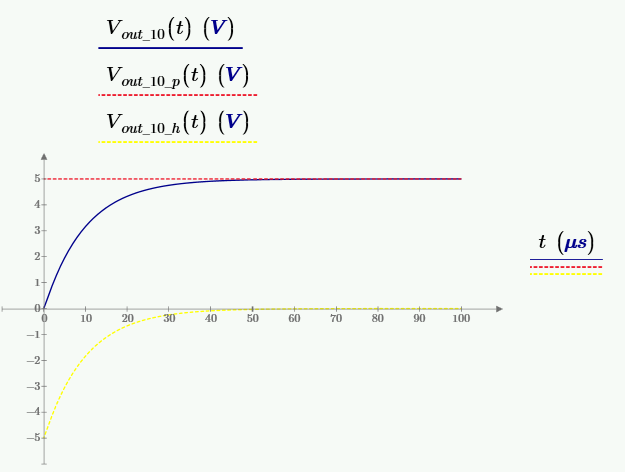
\includegraphics[height=5cm]{P_Fig/figur14_ana2graf10K}
  \caption{grafisk afbildning af $V_{out}{10}$}
  \label{graf10K}
 \end{center}
\end{figure}



\input{P_Tex/Ana2_kurveform1K}
\newpage
\subsubsection*{5. Bestem den maksimale værdi af Vout i de to tilfælde.}

For at finde den maksimale værdi af $V_{out}$ for de 2 grafer, kan det ved 1 k$\Omega$ måles ud fra grafen, mens det ved 10 k$\Omega$ både kan beregnes og måles.

$V_{max}$ for 1 k$\Omega$ = 5.766, som det også kan ses på nedstående graf. 

\begin{figure}[h]
 \begin{center}
  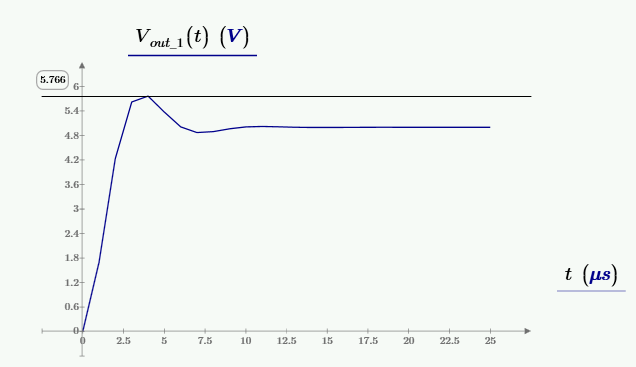
\includegraphics[height=5cm]{P_Fig/figur16_ana2graf1Kmax}
  \caption{$V_{max} 1 k\Omega$}
  \label{max1K}
 \end{center}
\end{figure}

Ved 10 k$\Omega$, kan dette beregnes ved at sætte tiden t til 100 procent i dette tilfælde vil det sige 100 $\mu s$

\begin{equation}
V_{max\_10} = V_{out\_10}(100\mu s)  = 5 V
\end{equation} 

Dette kan også ses på nedenstående graf:

\begin{figure}[h]
 \begin{center}
  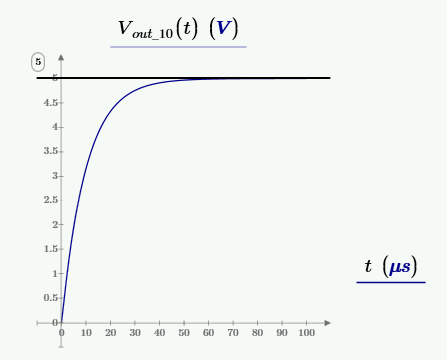
\includegraphics[height=5cm]{P_Fig/figur17_ana2graf10Kmax}
  \caption{$V_{max}$ 10 k$\Omega$}
  \label{max10K}
 \end{center}
\end{figure}